\newpage
\section{Funcionamiento del sistema}
El sistema funciona en un horario determinado correspondiente al horario escolar. Por fuera de ese horario el sistema permanece inactivo y las puertas cerradas con llave.
Durante los horarios de ingreso, las puertas permanecen abiertas para evitar \enquote{cuellos de botella} por parte de los alumnos, pero una vez iniciado el periodo de clases, las puertas permanecen cerradas. Del lado de afuera se debe instalar un manijón que no permita que se accione el resbalón, ya que este lo acciona un destrabador eléctrico comandado por el sistema. Del lado interior se coloca un picaporte, que permita el egreso en todo momento por motivos de seguridad ante una posible evacuación.
En casos de fallas del suministro energético, cuando el destrabador no pueda accionarse, basta con accionar el resbalón desde dentro con el picaporte o desde fuera con la llave.

En caso de que un visitante externo, por ejemplo el tutor de un alumno, visite la escuela, al tocar el pulsador del timbre de alguna de las puertas se le toma una fotografía que llega al dispositivo movil de la persona a cargo, quien decide si comandar o no una apertura. El tibre sonoro debe seguir funcionando normalente.

El personal de la institución contará con credenciales de acceso en formato de tags NFC, con los que podrán acceder sin mediación humana. El sistema deberá llevar registro de cada acceso por cualquiera de los dos medios mencionados. 


\subsection{Arquitectura del sistema}
El sistema se compone de un nodo servidor implementado en una \textit{single board computer} (SBC) comunicado con tres nodos llamdados terminales, construidos en base a microcontroladores, ubicados físicamente en cada punto de acceso. El servidor gestiona las comunicaciones, los registros, los permisos de acceso y por supuesto, comanda a los terminales. Los terminales son los que comandan, bajo demanda del servidor, el desbloqueo de las puertas mediante sendos relés que accionan los destrabadores eléctricos. También controlan las cámaras que toman las fotografías del exterior y los sensores NFC para transmitir la información de estos al seridor. 

Existen dos canales de comunicación entre nodos:

\begin{itemize}
    \item Comunicación serial cableada mediante protocolo RS-485 para el flujo de comandos, configuraciones y eventos, ya que es un estandar robusto utilizado en la industria, de velocidades considerables y pensado para grandes distancias.
    \item Conexión a la red local, en el caso de los terminales via WiFi, mientras que el servidor puede conectarse via wifi o mediante cable de red si fuera posible, para transmitir las fotografías tomadas, dado que su transmición no es crítica en tiempo y que una fotografía se corresponde a un volumen de datos mayor que puede congestionar el canal principal.
\end{itemize}

 \begin{figure}[ht]
	\centering
	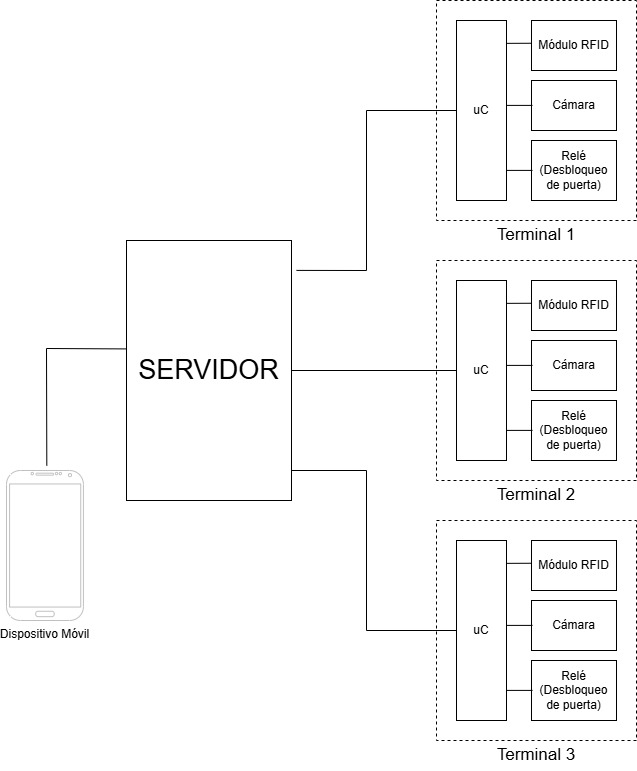
\includegraphics[width=0.7\textwidth]{img/DB1.jpeg}
	\caption{Diagrama de bloques del sistema}
	\label{fig:DB}
\end{figure}

\subsection{Actores del sistema}
El sistema reconoce tres tipos de actores humanos.

Los \textbf{accesos autorizados} son aquellos que cuenten con una credencial o \enquote{tag} nfc autorizado y puedan acceder al presentarlo frente al lector. El lector debe validar la identidad del tag mediante contraseña, recolectar la identificación y contador de accesos y enviarla al servidor, para que este contraste con la lista de tags permitidos y responda con la orden de apertura o de no apertura. El Funcionamiento de la lectura y validación se detalla en la sección (...).
El sistema debe tener capacidad para al menos 50 accesos autorizados, ya que representan al personal de la escuela (docente y no-docente) compuesto de alrededor de 30 personas. Se deja capacidad de reserva para cambios, incorporaciones y repuestos. 

Los \textbf{visiantes externos} son aquellas personas que no tienen autorización de ingresar fuera del horario de apertura. Estos, al pulsar el boton del timbre, son fotografiados por la cámara del terminal. La fotografía es enviada hacia el servidor, el cual lo envía hacia el dispositivo móvil donde un usuario final valida la identidad del visitante y concede o no el acceso. 

Los \textbf{usuarios finales} son aquellos con acceso a la interfaz de usuario de los dispositivos móviles. Para acceder a la interfaz estos deben loguearse con credenciales (usuario y contraseña). Según las credenciales pueden tener distintos roles. 
El más básico es el de usuario, cuya sesión permanece abierta en el dispositivo a menos que se cierre explícitamente o que se reabra en otro dispositivo. Este rol permite solo acciones básicas tales como comandar aperturas o solicitar fotografías. Este rol está dedicado al personal no docente, directivo o administrativo. El sistema admite hasta 6 usuarios con este rol.
Ciertos usuarios puden, mediante credenciales extra, abrir una sesión temporal de administrador, este rol permite configurar credenciales y añadir autorizaciones de accesos. Estas credenciales pertenecen solo a los directivos.
Finalmente, queda un rol de desarrollador al cual se accede con otras credenciales mediante un comando no disponible en el menú. Este rol no está pensado para el personal de la institución sino a quienes esten a cargo de la instalación y el mantenimiento del sistema, y permite realizar acciones simples sobre este sin la necesidad de acceder al servidor mediante SSH.

\subsection{Interfaces de usuario}

La interfaz principal para los usuarios finales funciona a travéz de un bot de la aplicación de mensajería instantanea \enquote{Telegram}, ya que la API es amigable con los desarrolladores y permite utilizar menúes y comandos de forma sencilla, además de que soluciona la conectividad con el exterior, sin tener que configurar manualmente puertos ni firewalls. Otra ventaja respecto a desarrollar una aplicación nativa es que no hay que hacer un desarrollo distinto para cada sistema operativo móvil.

El bot es en esencia un programa que se ejecuta permanentemente en el servidor y mediante llamadas a API recibe, procesa y envía mensajes al chat del bot.

Los registros históricos de accesos se dan en formatos legibles y se cargan diariamente a google drive mediante su API. Esto permite un fácil acceso a los datos y un ahorro de memoria del servidor al almacenar en la nube.

\subsection{Requerimientos del sistema}

Los requisitos temporales del sistema no son estrictos al punto de requerir una respuesta en tiempo real; sin embargo, el uso de este debe percibirse fluido para los actores.

Se establece entonces que el tiempo dé respuesta para los accesos autorizados debe estar en el orden de los dos segundos, contando desde que el tag se presenta ante el sensor hasta que se acciona el relé que destraba la puerta. 

En el caso del acceso de visitantes externos, el tiempo de respuesta se enmascara con la demora de la reacción humana, por lo que se establece una respuesta del orden de los cinco segundos del sistema para enviar la foto al usuario final, y del mismo orden para la apertura desde el comando manual, no pudendose controlar el tiempo de respuesta del usuario. 

Otro requerimiento es la robustez frente a fallas del suministro energético y la conexión a internet. Para eso se propone conectar el servidor a una unidad UPS para mantenerlo activo ante cortes de energía, aunque sin funcionamiento. El sistema se habilita solo en un horario determinado, en caso de un desfazaje del reloj del servidor, por ejemplo por un reinicio sin conexión a internet para ponerse en hora, se puede mediante un tag especial forzar el funcionamiento del sistema fuera de horario, al menos hasta que se retome la conectividad y el sistema vuelva a funcionar con normalidad.

El último requerimiento crítico es el de seguridad del sistema, el cual se abarca en la sección correspondiente (...).